\documentclass[a4paper,12pt]{article}

\usepackage{amsthm,amsmath,natbib,vmargin}

\usepackage[ansinew,utf8]{inputenc}

\usepackage{multirow,colortbl,color,array}

\usepackage[brazil]{babel}

\usepackage{bm}

\usepackage{graphicx}

\usepackage{natbib}


\usepackage{setspace}

\bibliographystyle{bbs}



%\pagestyle{headings}

%\theoremstyle{plain}

%\newtheorem{teo}{Teorema}[section]

\definecolor{gray}{rgb}{0.8,0.8,0.8}



\usepackage{subfigure}

\usepackage[T1]{fontenc} 

\usepackage{ae}

\usepackage[table,xcdraw]{xcolor}

\usepackage{amsmath}

\usepackage{blindtext}

\usepackage{scalefnt}

\usepackage{multirow}

%\usepackage{indentfirst}

\usepackage[a4paper,left=6cm,right=0cm,top=5cm,bottom=0cm]{geometry}

\usepackage[]{xcolor}

\usepackage{makeidx}

\usepackage{multicol}

\usepackage{float}

\usepackage{scalefnt} %muda tamanho da letra
\usepackage[absolute]{textpos}
\usepackage{pdfpages}
\newcommand*\NewPage{\newpage\null\newpage}
\usepackage{parskip}

%\usepackage[font=small,skip=0pt]{caption}

\usepackage{indentfirst}

\setlength{\parindent}{1.25cm}
\setstretch{1.5}



\begin{document}

\cleardoublepage
%___________________________________CAPA____________________________________
\pagestyle{empty}
\newpage

 \begin{center}
 \includegraphics[height=1.5cm,keepaspectratio]{unb}\\
 {\Large Universidade de Brasília\\
 IE - Departamento de Estatística\\
 Estágio Supervisionado 1}
 \vskip 10em
 {\Large \textbf{Análise de Sobrevivência para Dados Grupados}}
 \par
 \vskip 5em

{\setlength{\baselineskip}{.5cm}
\textbf{Daniel Lima Viegas}
\par}
\vskip 5em

\begin{flushright}

\vskip 2em
\small Orientador: Prof.ª Juliana Betini Fachini Gomes
\end{flushright}

\vskip 6em
{\setlength{\baselineskip}{.5cm}
Brasília\\
Setembro de 2017}

 \end{center}
 \NewPage
 
 
 %_________________________________Folha de rosto______________________________
 
\begin{center}
Daniel Lima Viegas
\end{center}


\vspace{12em}

{\Large \textbf{Análise de Sobrevivência para Dados Grupados}}


\begin{textblock*}{3.22in}(12cm, 14cm)
 \begin{minipage}[t]{9cm}
\vspace{8em}
    Orientadora:\\
  Profª. Drª. \textbf{Juliana Betini Fachini Gomes}
 \vspace{6em}

Monografia apresentada para a obtenção do título de Bacharel em Estatística.
\end{minipage}
\end{textblock*}
\vspace{28em}
\begin{center}
Brasília\\2018
\end{center}

 \NewPage
%___________________________________SUMÁRIO____________________________________

\tableofcontents
\NewPage

%__________________________________INTRODUÇÃO__________________________________
\newpage
\pagestyle{plain}
\section{Introdução}
\noindent

A análise de sobrevivência é um tópico importante utilizado em diversas áreas, como biologia, engenharia, medicina, entre outros. O principal objetivo desta análise é explicar ou predizer o tempo até a ocorrência do evento estudado, esse tempo é chamado de tempo de falha. A principal diferença desta técnica de modelagem para as demais é a capacidade de levar em consideração também os tempos em que não foi possível observar o evento de interesse, esse tipo de ocorrência é chamado de censura.

Dentre os tipos de censuras existentes, a mais genérica é a censura intervalar. Esse tipo de censura ocorre quando não é possível determinar o tempo de ocorrência, mas se tem o intervalo de tempo onde ele ocorreu. Por exemplo, no estudo sobre o tempo até uma lâmpada queimar, deixa-se a lâmpada ligada até que ela queime, em um dia, ela está funcionando, o pesquisador sai da área onde está acontecendo o experimento e quando retorna, a lâmpada está queimada. Neste caso, sabe-se que o intervalo de tempo onde a lâmpada queimou é entre o tempo em que o pesquisador saiu e o que ele voltou. O objetivo deste trabalho é estudar o comportamento de dados grupados, que é um caso particular da censura intervalar.

Em diversos estudos de sobrevivência, estuda-se o relacionamento de covariáveis e o tempo, tendo o objetivo de realizar as análises estatísticas e tentando encontrar o melhor uso dessas variáveis para a criação de um modelo de regressão para dados censurados.

O trabalho possui como objetivo, sugerir um modelo para dois bancos de diferentes áreas utilizando a metodologia de dados grupados. Um dos bancos foi utilizado no estudo de \cite{Barreto} na área da saúde e foi cedido pela Universidade Federal da Bahia. O outro banco de dados é um banco de dados na área da educação cedido pela Universidade Estadual da Paraíba.
\newpage
%_________________________________Revisão de Literatura__________________________
\section{Revisão de Literatura}

A fim de dar fundamento teórico ao trabalho na área de análise de sobrevivência, serão apresentados, a seguir, conceitos e notações presentes nas literaturas do tema.

\subsection{variável resposta e censuras}
Chama-se evento de interesse, aquilo que se deseja encontrar informações sobre a ocorrência. Na análise de sobrevivência, esse evento pode ser a morte de um indivíduo, a cura, um casamento, divórcio ou funcionamento de um dispositivo ou componente de uma máquina. Em análise de sobrevivência, a variável resposta é geralmente o tempo até a ocorrência de um evento de interesse, sendo esse tempo denominado tempo de falha.%citar colosimo;giolo%

A principal característica dos dados de sobrevivência é a presença de censuras, ou seja, observações que por algum motivo não consegue-se determinar o tempo com precisão. Existem três tipos principais de censura, a mais usual é a censura à direita, esta censura acontece quando não se consegue registrar a ocorrência do evento de interesse. Em estudos médicos que analisam o tempo desde a obtenção da doença até a morte do paciente, por exemplo, este tipo de censura acontece quando o paciente é curado, morre por outra razão ou simplesmente não se pode mais observar tal paciente. Este tipo de censura tem três tipos de classificação:

\begin{itemize}
	\item Censura do Tipo I: acontece quando a pesquisa tem um tempo pré-determinado. Ao final do estudo, as observações que não falharam são consideradas censuras. Nesse tipo de estudo, o percentual de censura é descrito como uma variável aleatória.
	
	\item Censura do Tipo II: É encontrada quando se obtém um determinado número de falhas dentro do experimento. Nesse tipo de experimento, o número de falhas deve ser determinado antes de começar o experimento, fazendo com que o número de falhas seja constante. O número de falhas, claramente deve ser menor do que o tamanho da amostra.
	
	\item Censura Aleatória: engloba os outros dois tipos de censura. Acontece quando alguns componentes não podem mais ser acompanhados ou quando o motivo da observação falhar é diferente do que interessa. Esta censura ocorre sem intervenção do pesquisador.

\end{itemize}

Além dessa censura também existem censuras importantes como a censura à esquerda e a censura intervalar. A censura à esquerda ocorre quando o evento ocorre antes do começo do experimento. Por exemplo, deseja-se observar o tempo até uma criança aprender a ler, porém no começo do estudo, algumas crianças podem já ter aprendido a ler sem saber exatamente o tempo em que ela aprendeu, isto é caracterizado como censura à esquerda. % citar colosimo giolo.

A censura intervalar pode ser dita como um caso genérico das outras censuras. Chama-se censura intervalar quando não se sabe o tempo em que ocorreu o evento de interesse
ocorreu, porém sabe-se que ele não ocorreu antes de um determinado tempo. Por exemplo, em um estudo médico é necessário que hajam visitas regulares para a detecção de certas doenças, tal como câncer. Nesse tipo de experimento, sabe-se que a doença apareceu antes do tempo de uma consulta (V), mas também sabe-se que ela apareceu depois de uma consulta (U), ou seja, a doença se manifestou no intervalo [U, V). Quando V = $\infty$
tem-se a censura a direita, e quando a o tempo U = 0, essa censura se torna a esquerda. Daí vem o conhecimento de caso genérico da censura.

\subsection{Tempo}

Como visto anteriormente, a variável resposta do experimento em questão é o tempo até o evento de interesse. Quando esse tempo pode assumir qualquer ponto real não-negativo, descreve-se essa variável como contínua. Esse é o tipo mais comum de variável na análise de sobrevivência, devido a grande diversidade de distribuições contínuas. %% talvez complemente, talvez seja desnecessário.

Em alguns casos, não faz sentido utilizar uma distribuição contínua para descrever o tempo, mas sim uma discreta. Pode-se ter como exemplo o tempo que um aluno leva para sair da universidade, pode levar 8 semestres, 9 semestres e assim por diante, ou seja, nunca vai levar um tempo real e sim um tempo pertencente aos naturais.%% Complementar

\subsection{Funções}

\subsubsection{Função densidade de probabilidade}

Dada uma variável aleatória contínua, não negativa, que represente o tempo de falha de uma observação. Chama-se função densidade, uma função \textit{f}, que descreva a probabilidade de um indivíduo falhar em um intervalo de tempo, quando esse intervalo tende a zero. Sendo assim, essa função descreve a distribuição de probabilidade ao longo do intervalo de zero a infinito.

A partir desta função, é possível obter-se a função de distribuição acumulada, denominada função \textit{F}. No caso contínuo, esta função é obtida a partir do cálculo da integral da função densidade sobre todo seu suporte. Ou seja, dada uma variável aleatória T:

\subsubsection{função densidade de probabilidade}

Uma função densidade de probabilidade é uma função que que satisfaz as seguintes condições:%citar Meyer 1983

\begin{enumerate}

	\item $f(x) \ge 0$ para todo $x$,
	\item $\int_{-\infty}^{+\infty} f(x)dx = 1$,
	\item para quaisquer a, b com $-\infty < a < b < +\infty$, teremos $P(a \le X \le b) = \int_a^b f(x)dx$.
\end{enumerate}
	 
		
\subsubsection{função de sobrevivência}

A função de sobrevivência é definida como a probabilidade de um indivíduo não falhar até um determinado tempo t, ou seja, é a probabilidade de uma observação viver além do tempo t. Dada uma variável aleatória T, contínua, não negativa. Pode-se descrever a função de sobrevivência como:

\begin{equation}
\label{eq}
	\begin{split}
		S(t) & = P(T > t) \\
		& = \int_t^{\infty} f(v)dv 
  	\end{split}
\end{equation} 

\subsubsection{Função de Risco}

Segundo \cite{Lawless}, esta funçao especifica a taxa de falha instantânea no tempo t dado que o indivíduo não falhou até esse tempo. Desta forma, é possível definir a função de risco como o limite da probabilidade de um indivíduo falhar no intervalo de tempo $[t, \delta t)$, supondo que esse indivíduo não falhou até o tempo t, dividida pelo comprimento do intervalo infinitesimal $\Delta t$. Com isso, é possível visualizar matematicamente a definição dessa função como:

\begin{equation} \label{eq:haz}
h(t) = \lim_{\Delta t \to 0}\dfrac{P(t \le T < t+\Delta t|T\ge t)}{\Delta t}.
\end{equation}

Além disso, também é possível estabelecer uma relação entre esta função, a função de densidade e a função de sobrevivência:

\begin{equation} \label{eq:haz_surv}
h(t) = \dfrac{-dS(t)}{dt}
\end{equation}


\subsubsection{Função de Risco Acumulado}

A função de risco acumulado é uma função que não possui uma interpretação simples, porém possui importância dentro do campo da análise de sobrevivência. Esta função, denotada como $H(t)$, pode ser definida como o logaritmo da função de sobrevivência multiplicado por menos um, ou seja:

\begin{equation} \label{eq:riskcum}
 H(t) = -log(S(t))
\end{equation}

Esta função também pode ser obtida através da Função de Risco:

\begin{equation} \label{eq:riskcum}
 H(t) = \int_0^t h(u)du.
\end{equation}

O gráfico desta função pode assumir algumas diferentes formas. Essas formas são utilizadas para determinar possíveis modelos probabilísticos que melhor se adequam aos dados. Com relação ao comportamento da função, o gráfico pode tomar as seguintes formas:
\begin{figure}[H]
  \centering
  \includegraphics[width=10cm]{risco_acum.png}
  \caption{Comportamentos da Função Risco Acumulada}
\end{figure}

\begin{itemize}
	\item A $\Rightarrow$ Função de risco constante é adequada.
	\item B ou C $\Rightarrow$ Função
risco é monotonicamente crescente ou decrescente, respectivamente.
	\item D $\Rightarrow$ Função risco tem forma de \textbf{U}.
	\item E $\Rightarrow$ Função risco tem comportamento unimodal.
\end{itemize}

\subsection{Estimadores da função de sobrevivência}

\subsubsection{Estimação simples}

A função de sobrevivência pode ser estimada amostralmente, como a proporção dos dados que não falharam até o tempo t. Esse estimador poderia ser escrito da seguinte forma:

$$ \hat{S}(t) = \dfrac{n^o \ de \ dados \ com \ tempo \ > \ t}{n^o \ total \ de \ individuos}, \forall \ t \ \in t\ge 0$$

Caso os dados sejam ordenados de forma crescente, pode-se representar a função de sobrevivência da seguinte forma:

$$ \hat{S}(t) = \dfrac{n_j - d_j}{n} $$

Onde $n_j$ é o número de indivíduos que podem falhar, $d_j$ é o número de indivíduos que que falharam no tempo e n é o número total de indivíduos.

\subsubsection{Kaplan-Meier}

Os estimadores apresentados acima, não podem ser usados nesse tipo de estudo porque não existe nenhuma forma de se incluir censuras.

O estimador a ser usado nesse trabalho será o estimador não-paramétrico de Kaplan-Meier. Esse estimador é muito popular em pesquisas que usam análise de sobrevivência. O estimador é escrito da seguinte forma:

$$ \hat{S}(t) = \prod_{j:t_{(j)}\le t} \dfrac{n_j - d_j}{n_j}$$

Onde, $n_j$ representa o número de dados em risco de falha, $d_j$ são os dados que falharam no tempo $t_j$, em que, $0 \le t_{(1)} \le \hdots \le t_{(n)}$, são os tempos distintos de falha. Esta técnica não utiliza covariáveis para a estimação, mas pode usar variável categóricas para verificar se as funções estimadas são diferentes. 

A representação gráfica desse método se comporta em uma função da forma de escada, uma vez que a estimação entre o tempo $t_{(j)}$ e $t_{(j+1)}$ é constante.


\subsection{Modelos de Probabilidade}

\subsubsection{Modelo Log-Logístico}

Para os casos onde T é uma variável aleatória contínua seguindo uma distribuição Log-Logística com parâmetro de escala $\alpha$ e de forma $\gamma$, sua função densidade de probabilidade é descrita como

\begin{equation}
  f(t) = \dfrac{\gamma\left(\dfrac{t}{\alpha}\right)^{\gamma - 1}}{\alpha\left[1+\left(\dfrac{t}{\alpha}\right)^{\gamma}\right]^2}, \hspace{1cm} t > 0
\end{equation}

Onde $\alpha$ e $\gamma$ são constantes, ambas maiores que 0. Com base na função densidade, é possível descrever a função de sobrevivência da variável aleatória T como:

\begin{equation} \label{eq: LLSurv}
  S(t) = \dfrac{1}{1 + \left(\dfrac{t}{\alpha}\right)^{\gamma}}
\end{equation}

E a partir desta função pode-se encontrar a função risco acumulado:

\begin{equation} \label{eq: HazLL}
H(t) = - \log{\dfrac{1}{1 + \left(\dfrac{t}{\alpha}\right)^{\gamma}}}
\end{equation}

Com relação ao comportamento da função de risco, quando $\gamma$ é menor que 1, esta é monótona decrescente, enquanto para valores maiores que 1 a função tem um comportamento monótono crescente.

A partir da função \ref{eq: LLSurv} ainda é possível definir a função de risco do modelo:

\begin{equation} \label{eq: hazLL}
h(t) = \dfrac{\gamma(t/\alpha)^{\gamma-1}}{\alpha[1+(t/\alpha)^\gamma]}
\end{equation}


\subsection{Método de Máxima Verossimilhança}

Para a estimação dos parâmetros da função de distribuição, e também para os parâmetros do modelo, existe uma grande variedade de formas para efetuar tal procedimento. Como a característica principal da análise de sobrevivência é a presença de censuras, o procedimento também deve incorporar tal característica. Por esse motivo, é descartado alguns métodos para a estimação.

Um método que consegue incorporar a censura é o método da máxima verossimilhança. Este método tem como objetivo encontrar o valor do parâmetro que maximiza a probabilidade da amostra observada ser encontrada. Este método mostra-se adequado por permitir a incorporação das censuras através da inclusão da função de sobrevivência para os tempos censurados, enquanto os tempos em que ocorreram falha, considera-se a função densidade.

Para os tipos de censura à direita mostrados, a função de máxima verossimilhança a ser maximizada pode ser descrita analíticamente e a menos de constantes, é dada por \cite{colosimo}:

\begin{equation} \label{eq:maxv1}
  L(\boldsymbol{\theta}) \propto \prod_{i=1}^n \left[f(t_i;\boldsymbol{\theta})\right]^{\delta_i} \left[S(t_i;\boldsymbol{\theta})\right]^{1-\delta_i},
\end{equation}

onde $\delta_i$ é a variável indicadora de falha e $\boldsymbol{\theta}$ é o vetor de parâmetros que serão estimados.

Para encontrar o estimador de máxima verossimilhança, deriva-se a função de verossimilhança, ou o log da função, em todos os parâmetros e iguala as funções resultantes a zero encontrando assim um valor para todos os parâmetros no vetor $\boldsymbol{\theta}$. Para a resolução do sistema são geralmente utilizados métodos computacionais de otimização numérica devido a grande complexidade dos cálculos. 


\subsection{Dados Grupados}

A análise de sobrevivência com censura intervalar, tem como caso particular os dados grupados. Essa particularidade acontece quando acontece um número excessivo de empates, ou seja, os tempos de vida se repetem diversas vezes. Este tipo de experimento pode ser encontrado em estudos de medidas repetidas longitudinais.

Para esse tipo de estudo, os tempos são separados em intervalos arbitrários e disjuntos isso significa que os intervalos não precisam ter o mesmo tamanho e que não podem haver interseções entre os intervalos. As funções utilizadas na análise, tais como função de sobrevivência e de risco são as mesmas utilizadas quando o tempo é contínuo.

A função de verossimilhança se diferencia da forma utilizada na análise de sobrevivência devido a agregação dos valores em intervalos. Segundo \cite{elisangela}, a função de verossimilhança para esse caso pode ser descrita como:

\begin{equation} \label{eq:like_group}
  \begin{split}
    L(\boldsymbol{\theta})  =  &\prod\limits_{j=1}^k\Bigg\{ \prod\limits_{i\in F_j} 1 - \dfrac{S(a_{j+1})}{S(a_{j})} \\
    & \times \prod\limits_{i\in R_j} \dfrac{S(a_{j+1})}{S(a_{j})} \\
    & \times \prod\limits_{i\in C_j} \left[\dfrac{S(a_{j+1})}{S(a_{j})}\right]^{1/2}\Bigg\},
  \end{split}
\end{equation}

\noindent onde, $\boldsymbol{\theta}$ é o vetor de parâmetros, k é o número de intervalos no estudo, $F_j$ é o grupo de individuos que falharam, $R_j$ é o grupo de indivíduos que sobreviveram, ou não falharam, nesse intervalo e $C_j$ são os individuos que foram censurados naquele intervalo. Os valores de $a_j$ e $a_{j+1}$ são os limites dos intervalos, sendo o primeiro o limite inferior e o segundo o superior.

\subsection{Resíduos de Cox-Snell}

Para avaliar a qualidade do ajuste do modelo, realiza-se o cálculo de medidas que possam mensurar essa qualidade. Por se tratar de modelos censurados, a análise de resíduos na análise de sobrevivência não são tão visualizáveis e por isso, existem diversas medidas de resíduos passíveis de serem utilizados. Esta subseção comenta os resíduos de Cox-Snell.

Segundo \cite{colosimo}, esses resíduos são obtidos através da função risco acumulada obtida pelo modelo ajustado:

\begin{equation} \label{eq:cox}
  \hat{e_i} = \hat{H}(ti|\boldsymbol{x})
\end{equation}

Os resíduos $\hat{e_i}$ devem seguir distribuição exponencial padrão (\cite{Lawless}). Cada tempo presente no banco de dados gera um resíduo, desta forma cada resíduo possui um indicador de censura. Para realizar a análise gráfica do modelo, calcula-se o estimador de Kaplan-Meier para a função de sobrevivência dos resíduos e cria o gráfico desta estimativa sobreposta pela curva de sobrevivência da distribuição exponencial padrão.

A qualidade do ajuste é determinada a partir da proximidade entre as duas curvas. Caso a curva gerada pelos resíduos aparente ter uma distribuição exponencial e sobrepor de forma satisfatória a curva gerada pela exponencial padrão, então diz-se que o modelo possui um bom ajuste.


%__________________________________METODOLOGIA__________________________________
\newpage
\section{Metodologia}
\noindent

\subsection{Material}

A fim de propor um modelo de regressão para dados grupados, irá ser utilizado um banco de dados cedido pelo Instituto de Saúde Coletiva da Universidade Federal da Bahia. Esses dados foram obtidos a partir de um estudo conduzido por Barreto et al.(1994). O banco de dados é formado por 1207 crianças com idade entre 6 e 48 meses no início do estudo, que receberam placebo ou vitamina A. Dentre as variáveis se encontra a variável tempo, que é o tempo entre a primeira dose de placebo ou vitamina A e a ocorrência de diarreia na criança, a variável idade(0 - < 24 meses, 1 - $\ge$ 24 meses), tipo de tratamento(0 - Placebo, 1 - Vitamina A) e a variável sexo(0 - Feminino, 1 - Masculino). Para o agrupamento dos tempos, foram utilizados os mesmos 12 intervalos obtidos por \cite{elisangela}.

Além deste, será utilizado um banco de dados cedido pela Universidade Estadual da Paraíba. Este é formado por informações de mais de 600 alunos do curso de química da UEPB e seu objeto de estudo é o tempo desde a entrada de um estudante até a evasão desse aluno. O banco tem o ano de entrada e o semestre de entrada de cada aluno e a partir daí o acompanhamento se segue até o acontecimento do evento de interesse, da censura ou do fim do tempo mínimo do aluno. Para a modelagem serão adotadas 6 covariáveis, sendo estas Sexo do aluno(0 - Masculino, 1 - Feminino), Turno(0 - Diurno, 1 - Noturno), Escola(0 - Privado, 1 - Publico), Ingresso(0 - Vestibular, 1 - ENEM), Idade(0 - < 19 anos, $\ge$ 19 anos), Origem(0 - Outras Cidades, 1 - Campina Grande). Para a separação dos intervalos, foi decidido que cada semestre seria um intervalo, sendo que os semestres vão de 0 a 12.

\subsection{Métodos}

\subsubsection{Modelo de Regressão Log-Logístico}

Nos estudos em sobrevivência, é comum utilizar modelos de regressão para entender se o tempo em estudo é bem explicado por alguma distribuição de probabilidade, nesse caso utiliza-se o método de máxima verossimilhança para encontrar os parâmetros da distribuição escolhida e verifica-se o ajuste de tal distribuição graficamente.

Além disso, pode-se desejar entender o comportamento da variável resposta segundo covariáveis. Nesse caso, utiliza-se uma reparametrização de um parâmetro da distribuição escolhida através de uma função de ligação. Para este trabalho, foi escolhida a distribuição Log-Logística e o parâmetro que será reparametrizado, será o parâmetro de escala citado na subseção 2.5.1.

A função de ligação tem como objetivo conectar as covariáveis com a variável resposta através de um preditor linear definido como o produto da matriz transposta de covariáveis com o vetor de parâmetros, tal que para um conjunto de covariáveis o parâmetro de escala presente na distribuição pode ser descrito como:

\begin{equation} \label{eq:lig}
  \alpha = g(\boldsymbol{\eta}) = \exp(\boldsymbol{x}^T\boldsymbol{\beta})
\end{equation}

Com isso, é possível reescrever as funções presentes em 2.5.1 para adaptá-las ao modelo de regressão Log-Logístico com covariáveis. As funções necessárias para a realização da modelagem será a função de sobrevivência e para calcular o resíduo de Cox-Snell será utilizada também a função risco acumulada.

A função de sobrevivência da distribuição Log-Logística adicionando as covariáveis pode ser descrita como:

\begin{equation} \label{eq: LLSurvMod}
  S(t) = \dfrac{1}{1 + \left(\dfrac{t}{\exp(\boldsymbol{x}^T\boldsymbol{\beta})}\right)^{\gamma}}
\end{equation}

E a partir desta, é possível encontrar a função risco acumulada:

\begin{equation} \label{eq: HazLLMod}
H(t) = - \log{\dfrac{1}{1 + \left(\dfrac{t}{\exp(\boldsymbol{x}^T\boldsymbol{\beta})}\right)^{\gamma}}}
\end{equation}

Para a estimação dos parâmetros do modelo é utilizada a função de verossimilhança. Utiliza-se o log desta função para a estimação dos parâmetros. Assim, utilizando a função \ref{eq:like_group} tem-se:

\begin{equation} \label{eq:like_groupMod}
  \begin{split}
  \log(L(\boldsymbol{\theta}))  =  &\sum\limits_{j=1}^k\Bigg\{ \sum\limits_{i\in F_j} \log\left[1 - \dfrac{S(a_{j+1}|\boldsymbol{x}_i)}{S(a_{j}|\boldsymbol{x}_i)}\right] \\
    & + \sum\limits_{i\in R_j} \log\left[\dfrac{S(a_{j+1}|\boldsymbol{x}_i)}{S(a_{j}|\boldsymbol{x}_i)}\right] \\
    & + \sum\limits_{i\in C_j} 0.5\times\log\left[\dfrac{S(a_{j+1}|\boldsymbol{x}_i)}{S(a_{j}|\boldsymbol{x}_i)}\right]\Bigg\}
\end{split}
\end{equation}

Finalmente, substituindo \ref{eq: LLSurvMod} em \ref{eq:like_groupMod}:

\begin{equation} \label{eq:like_groupMod}
  \begin{split}
    l(\boldsymbol{\theta}) = & \sum\limits_{j=1}^k\Bigg\{ \sum\limits_{i\in F_j} \log\left[1 - \dfrac{1 + \left(\dfrac{a_j}{\exp(\boldsymbol{x}^T\boldsymbol{\beta})}\right)^{\gamma}}{1 + \left(\dfrac{a_{j+1}}{\exp(\boldsymbol{x}^T\boldsymbol{\beta})}\right)^{\gamma}}\right] \\
    & +\sum\limits_{i\in R_j} \log\left[\dfrac{1 + \left(\dfrac{a_j}{\exp(\boldsymbol{x}^T\boldsymbol{\beta})}\right)^{\gamma}}{1 + \left(\dfrac{a_{j+1}}{\exp(\boldsymbol{x}^T\boldsymbol{\beta})}\right)^{\gamma}}\right] \\
    & + \sum\limits_{i\in C_j} 0.5\times \log\left[\dfrac{1 + \left(\dfrac{a_j}{\exp(\boldsymbol{x}^T\boldsymbol{\beta})}\right)^{\gamma}}{1 + \left(\dfrac{a_{j+1}}{\exp(\boldsymbol{x}^T\boldsymbol{\beta})}\right)^{\gamma}}\right]
  \end{split}
\end{equation}

\noindent em que, $l(\boldsymbol{\theta}) = \log(L(\boldsymbol{\theta}))$. A partir desse ponto, deve-se seguir o processo de otimização citado na subseção 2.6, ou seja, calcula-se a derivada da função log-verossimilhança e encontra o ponto onde todos as equações geradas são iguais a zero. Por se tratarem de diversos parâmetros, são utilizados procedimentos de otimização numérica para se estimar tais valores. Para estes procedimentos será utilizado o \textit{software} R(\cite{R}).

Para a avaliação da modelagem será utlizado o método gráfico dos resíduos de Cox-Snell. Esses resíduos são gerados a partir da função risco acumulada da distribuição em questão gerada pelos parâmetros do modelo. Os resíduos de Cox-Snell, nesse caso serão dados por \ref{eq: HazLLMod}.


\newpage

\section{Resultados e Discussão}

\subsection{Suplementação de Vitamina}
\subsubsection{Análise Descritiva}

Para iniciar a análise dos resultados do banco de suplementação de Vitamina A, será realizada a análise exploratória do tempo e das covariáveis. Primeiro, é realizado um histograma da variável tempo incluindo todos os tempo de censura e de falha.

\begin{figure}[H]
  \begin{center}
    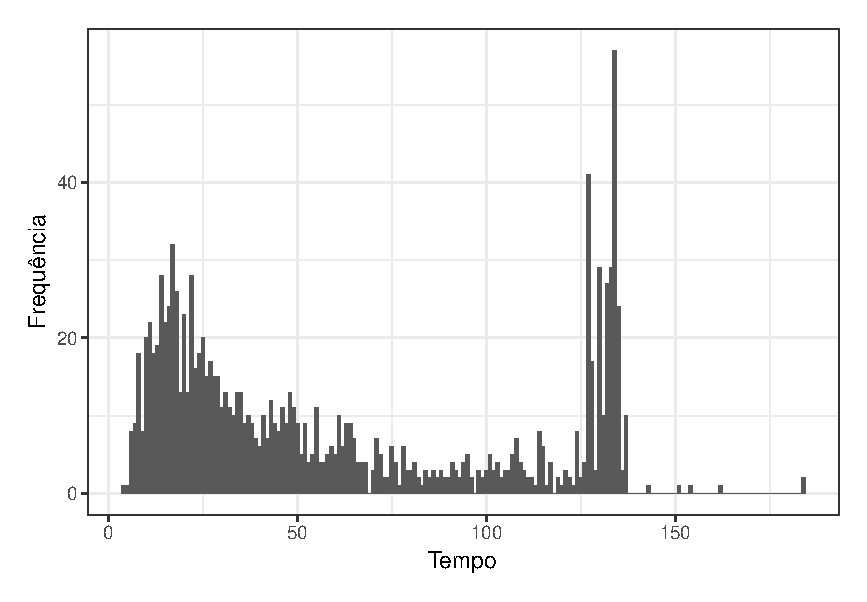
\includegraphics[width=10cm]{hist_vit}
    \caption{Histograma dos dados de Vitamina.}
  \end{center}
\end{figure}

Pelo gráfico é possível notar que em grande parte dos tempos existem muitos empates nos tempos do estudo, ou seja, muitos tempos se repetem em diversas observações e essa é uma justificativa do porquê utilizar a metodologia de dados grupados.

Outro procedimento passível de ser realizado para a análise exploratória é a estimação da função de sobrevivência através de Kaplan-Meier. Na Figura 3 é possível notar que o decréscimo da função é mais rápido no começo da função e vai diminuindo conforme vai passando o tempo. Também é possível perceber uma grande concentração de censuras mais ao final do estudo. 

\begin{figure}[H] \label{fig:surv_vit}
  \begin{center}
    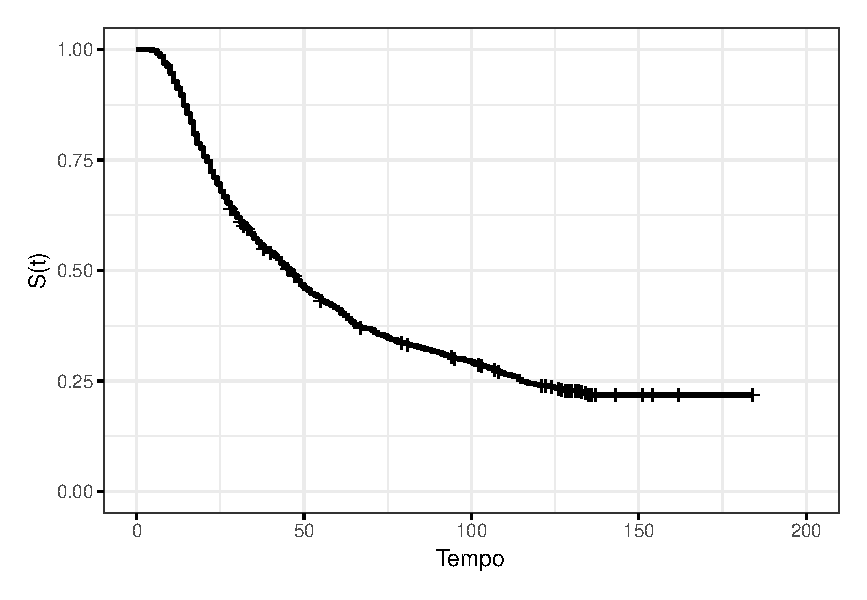
\includegraphics[width=10cm, height = 6cm]{surv_vit}
    \caption{Função de Sobrevivência Estimada.}
  \end{center}
\end{figure}

Para a realização do estudo utilizando a metodologia de dados grupos, o tempo de sobrevivência foi grupado em 12 intervalos, como dito na seção 3.1. A Tabela 1 apresenta os intervalos escolhidos, o número de falhas, o de censuras e o número de indivíduos sob risco.

\begin{table}[H]
\centering
\caption{Descrição dos tempos de vida utilizando os intervalos grupados}
\begin{tabular}{cccc}
\hline
Intervalo & Número de falhas & Número de censuras & Número sob risco \\
\hline
[4, 14)   & 124 & 0 & 1207 \\

[14, 18)  & 106 & 0 & 1083 \\

[18, 23) & 103 & 0 & 977 \\

[23, 29) & 100 & 1 & 874 \\

[29, 37) & 92 & 3 & 773 \\

[37, 48) & 92 & 6 & 678 \\

[48, 61) & 90 & 1 & 580 \\

[61, 73) & 67 & 1 & 489 \\

[73, 90) & 46 & 3 & 421  \\

[90, 108) & 49 & 6 & 372 \\

[108, 126) & 10 & 11 & 317 \\

[126, 185) & 10 & 250 & 260\\
\hline
\end{tabular}
\end{table}


Após observar o comportamento da função de sobrevivência estimada considerando apenas o tempo, pode-se incluir covariáveis uma a uma e avaliar a diferença entre as curvas de sobrevivências geradas.

\begin{figure}[H]
  \begin{center}
    \includegraphics[width=10cm, height = 6cm]{surv_idade_vit_1}
    \caption{Função de Sobrevivência Estimada separada por idade.}
  \end{center}
\end{figure}

Através da Figura 4, é perceptível que existe uma certa diferença entre os dois grupos. Crianças com idade maior ou igual 24 meses aparentam ter uma maior probabilidade de sobrevivência que crianças com idade menor que 24 meses.

Analisando a covariável sexo pela Figura 5, percebe-se que na maior parte do tempo, as curvas estão se sobrepondo o que indica que a variável não é muito significativa para o modelo, ou seja, o fato de ser menino ou menina não aparenta interferir significativamente na probabilidade de sobrevivência da criança.

\begin{figure}[H]
  \begin{center}
    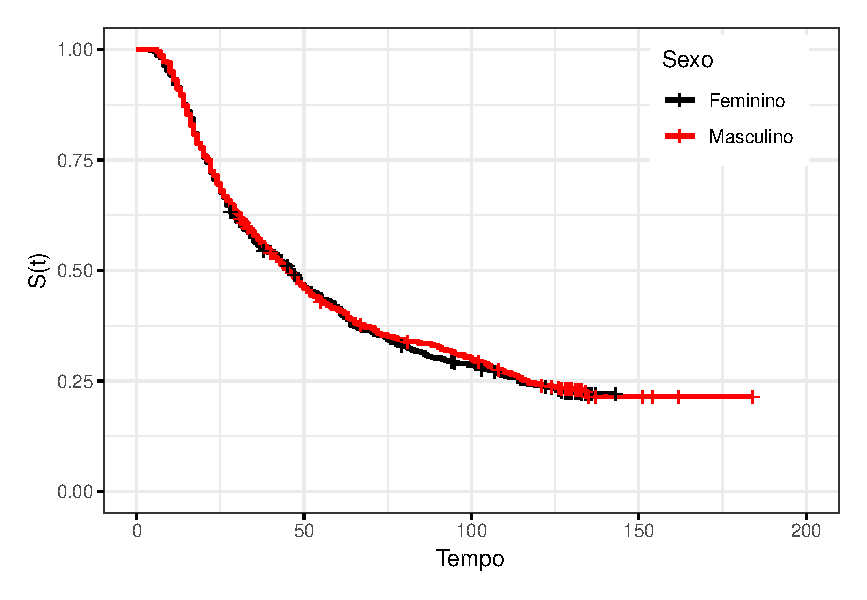
\includegraphics[width=10cm, height = 6cm]{surv_sexo_vit}
    \caption{Função de Sobrevivência Estimada separada por sexo.}
  \end{center}
\end{figure}

A Figura 6 mostra o efeito do tipo de tratamento na variável tempo. As curvas apresentam um certo distanciamento conforme o tempo passa. As crianças que foram suplementadas com Vitamina A aparentam ter probabilidade de sobrevivência maior que as que foram suplementadas com Placebo.

\begin{figure}[H]
  \begin{center}
    \includegraphics[width=10cm, height = 6cm]{surv_trat_vit}
    \caption{Função de Sobrevivência Estimada separada por tipo de tratamento.}
  \end{center}
\end{figure}


O gráfico da função risco acumulada é utilizada para identificar um comportamento na função de risco e desta forma auxilia na suposição de um modelo adequado, como foi visto na seção 2.3.5.

\begin{figure}[H] \label{fig:surv_vit}
  \begin{center}
    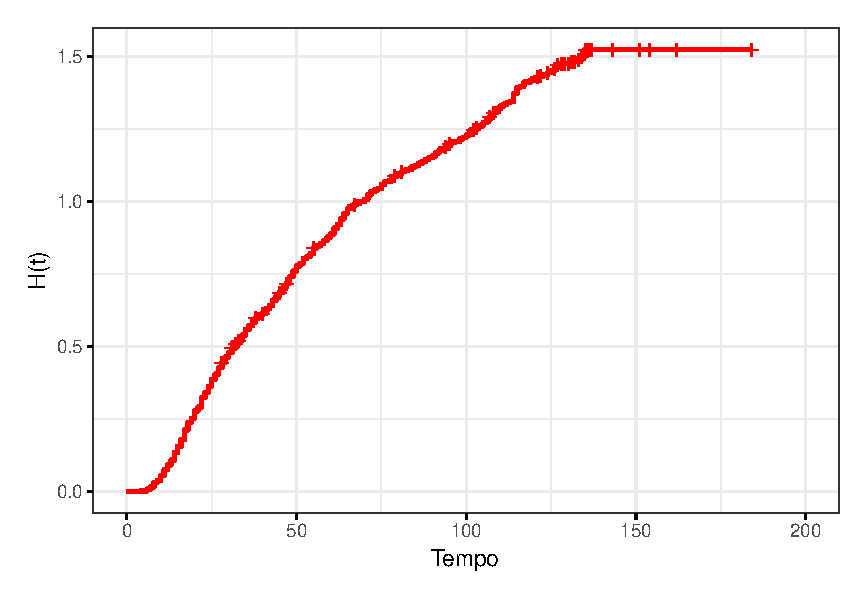
\includegraphics[width=10cm]{cum_haz_vit}
    \caption{Função de Sobrevivência Estimada.}
  \end{center}
\end{figure}

Observando o gráfico, nota-se que o comportamento é muito similar ao (C) da seção 2.3.5 o que indica que a função de risco tem um comportamento decrescente. Desta forma, uma distribuição de probabilidade possível seria a Log-Logística.

\subsubsection{Modelagem}

Tendo como objetivo encontrar um modelo que explique bem a variável tempo de sobrevivência, nesta seção serão tratados a modelagem, a seleção de variáveis e a análise de resíduos.

Ao realizar a modelagem sem considerar nenhuma covariável e apenas estimar os parâmetros da distribuição Log-Logística, é possível realizar a comparação entre a função distribuição estimada pela função de máxima verossimilhança adapatada para o método de dados grupados e a função de sobrevivência estimada por Kaplan-Meier.

\begin{figure}[H] \label{fig:surv_vit}
  \begin{center}
    \includegraphics[width=10cm]{mod_vazio_vit}
    \caption{Função de Sobrevivência Estimada.}
  \end{center}
\end{figure}

Ao que se pode observar a curva da distribuição estimada(curva suave em preto) se sobrepõe a boa parte da função estimada por Kaplan-Meier o que indica que a distribuição explica bem a variável resposta independente de covariáveis. Na Tabela 2 estão presentes os valores das estimativas de cada parâmetro, assim como seus erros padrões.

\begin{table}[H]
\centering
\caption{Estimativas dos parâmetros da distribuição log-logística sem covariáveis.}
\begin{tabular}{c|cc}
\hline
Parâmetro & Estimativa & Erro Padrão \\
\hline
$\alpha$ & 44,57 & 1,98  \\

$\gamma$ & 1,23 & 0.045 \\
\hline
\end{tabular}
\end{table}

Outra parte da modelagem que será realizada é a inclusão de covariáveis para verificar quais variáveis são significativas ao tentar explicar o tempo. Para isso, mais uma vez será realizada a estimação dos parâmetros através da função de máxima verossimilhança utilizando a metodologia em questão e para a inclusão das covariáveis, será utilizada a função de ligação $g(\eta) = \exp(\boldsymbol{x}^T\boldsymbol{\beta})$. Assim, o parâmetro $\alpha$ pode ser escrito, utilizando todas as variáveis explicativas, da seguinte forma:

\begin{equation} \label{eq:conn_vit}
\alpha_i = exp(\beta_0 + \beta_1Idade_i + \beta_2Tratamento_i + \beta_3Sexo_i)
\end{equation}

Como pode ser observado na equação \ref{eq:conn_vit} as variáveis possuem o nome do que indicam. A Tabela 3 mostra os parâmetros estimados do modelo completo, assim como seus erros padrão e os p-valores com relação a significância do parâmetro.

\begin{table}[H]
\centering
\caption{Estimativas dos parâmetros do modelo completo.}
\begin{tabular}{c|ccc}
\hline
Parâmetro & Estimativa & Erro Padrão & p-valor \\
\hline
Intercepto & 3.24 & 0,087 & < 0,001 \\

Idade & 0,83 & 0,082 & < 0,001 \\

Tratamento & 0,16 & 0,08 & 0,04 \\

Sexo & 0,05 & 0,07 & 0,48 \\

$\gamma$ & 1,23 & 0.045 & - \\
\hline
\end{tabular}
\end{table}

A tabela acima mostra que todas as covariáveis foram significantes menos a variável sexo. O Teste da Razão de Verossimilhança indica que o modelo retirando essa variável é adequado. A partir disto, é criada a Tabela 4 com as informações dos parâmetros utilizados nesse novo modelo.

\begin{table}[H]
\centering
\caption{Estimativas dos parâmetros do modelo completo.}
\begin{tabular}{c|ccc}
\hline
Parâmetro & Estimativa & Erro Padrão & p-valor \\
\hline
Intercepto & 3,28 & 0,075 & < 0,001 \\

Idade & 0,83 & 0,082 & < 0,001 \\

Tratamento & 0,16 & 0,08 & 0,04 \\

$\gamma$ & 1,31 & 0.047 & - \\
\hline
\end{tabular}
\end{table}

Pelos resultados, tem-se que todos as variáveis são significativas tanto a um nível de 5\%. Além disso, o Teste da Razão de Verossimilhança indica que não devem ser retiradas nenhuma variável do modelo e por isso, esse foi escolhido como candidato ao modelo final. Pelos resultados dos parâmetros, percebe-se que o modelo apresenta taxa de falha unimodal devido a estimação do parâmetro $\gamma$ ser 1,31. A estimativa do parâmetro de idade indica que crianças com idade maior que 24 meses possuem maior probabilidade de sobrevivência. Quanto a variável tratamento, quem apresenta maior probabilidade são as que crianças que foram suplementadas com Vitamina A.

Com o objetivo de verificar a qualidade do ajuste do modelo, realiza-se a análise gráfica de resíduos de Cox-Snell. A Figura 9 mostra os resíduos gerados pelo candidato a modelo final.

\begin{figure}[H] \label{fig:surv_vit}
  \begin{center}
    \includegraphics[width=10cm]{mod_vazio_vit}
    \caption{Resíduos de Cox-Snell.}
  \end{center}
\end{figure}

No gráfico, é possível perceber que a curva do resíduo se aproxima bem da curva da exponencial padrão. Com isso, percebe-se que o modelo explica bem o tempo e por isso esse modelo pode ser considerado como modelo final.

\subsection{Evasão Curso de Química}
\subsubsection{Análise Descritiva}

A fim de explorar inicialmente os dados, é realizada um histograma da variável tempo sem considerar nenhuma covariável nem a indicação de censura.

\begin{figure}[H]
  \centering
  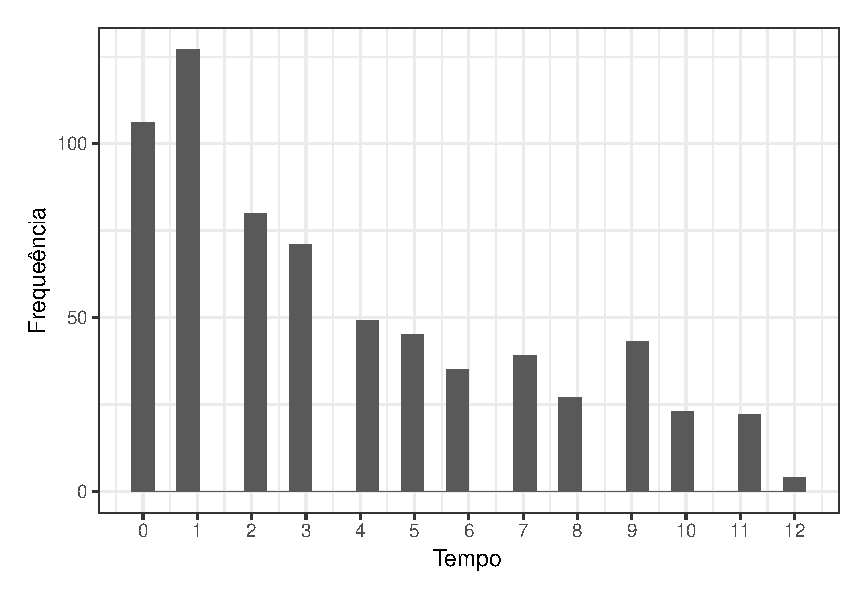
\includegraphics[width=10cm]{quim_hist}
  \caption{Histrograma dos tempos de evasão}
\end{figure}

Como é possível observar, devido ao fato de que os alunos só podem permanecer na universidade por 12 semestres existem muitos empates dentro desse modelo, justificando assim o uso da metodologia de dados grupados.

Para verificar a forma da estimativa da função de sobrevivência, é realizada a estimação por Kaplan-Meier e faz-se o gráfico dessa estimativa.

\begin{figure}[H]
  \centering
  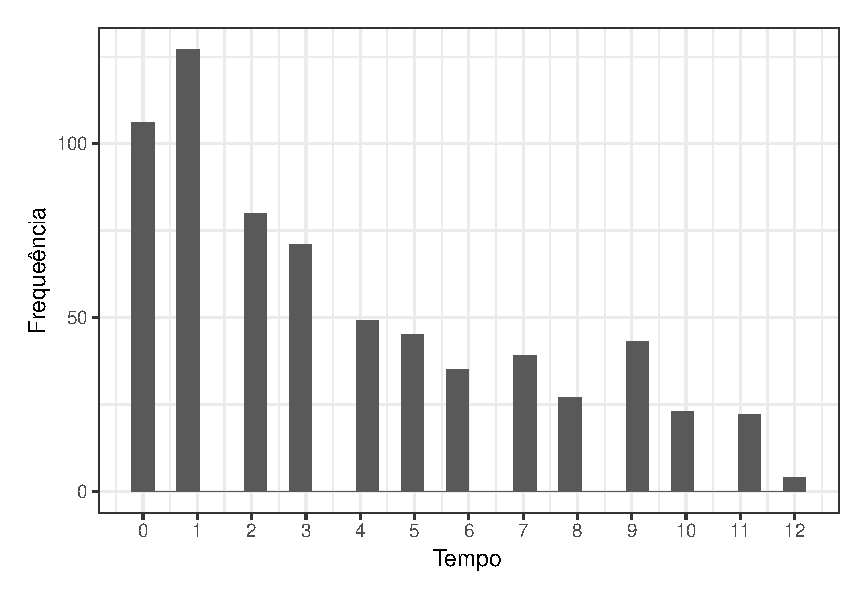
\includegraphics[width=10cm]{quim_hist}
  \caption{Histrograma dos tempos de evasão}
\end{figure}


\newpage
\addcontentsline{toc}{section}{Referências}



\bibliography{referencias.bib}
\nocite{*}


\end{document} 